%!TEX root = ../template.tex
%%%%%%%%%%%%%%%%%%%%%%%%%%%%%%%%%%%%%%%%%%%%%%%%%%%%%%%%%%%%%%%%%%%%
%% chapter3.tex
%% NOVA thesis document file
%%
%% Chapter with lots of dummy text
%%%%%%%%%%%%%%%%%%%%%%%%%%%%%%%%%%%%%%%%%%%%%%%%%%%%%%%%%%%%%%%%%%%%

\typeout{NT FILE chapter3.tex}%
\label{cha:neurobehav}

% (fold)
\newcommandx{\obs}[2][1=]{\todo[linecolor=lightgray,backgroundcolor=lightgray,bordercolor=white,#1]{#2}}
\NewDocumentCommand{\dummyref}{m}{\textcolor{red}{#1}}
% (end)

\chapter{Non-linear mixed representations improve behavioral readouts} 
% Decoding behavior from Purkinje-cells suggests non linear (...) 

\pagebreak

\section{Abstract}
\section{Introduction}


\begin{compactitem}
    \scriptsize
    \item Purkinje cells are required for coordination
    \item Purkinje cell simple spike rate encodes kinematics and position
    \item Population providing readouts (DCN convergence + Shadmehr)
    \item Recent mixed selectivity proposes efficient encoding schema
\end{compactitem}

\vspace{10pt}

Based on histological and circuit characterization studies, the cerebellum is proposed to be a key structure involved in learning. Within this framework, Purkinje cells are regarded as the primary computational units of the cerebellum, forming the foundation of the Albus-Marr-Ito hypothesis (\dummyref{Ito?}).
\obs{This should be in chapter 1 (intro)}
During locomotion, the timing of strides across all limbs must be precise to maintain stability, and any motor errors, whether internal or external, must be flexibly compensated for. Internal errors are defined as those arising from motor noise, while external errors refer to unexpected changes in the environment (\dummyref{ref wolpert kawato}).

Cerebellar lesions are known for resulting in movement ataxia, in which humans or animals' capability to produce well-timed, coordinated movements is impaired. Loss of function in the cerebellum matches what would be expected if the motor system could no longer estimate the sensorimotor consequences of motor commands (\textcolor{red}{Bastian ref}). More specifically, localized perturbation of Purkinje cells that project to a single cerebellar nucleus results in abolished learning of a locomotor paradigm without completely compromising the animals' ability to walk (\cite{darmohray_spatial_2019}). This and similar findings \dummyref{refs on Purkinje cell transient impairment} are consistent with the idea of Purkinje cells as cerebellar computational units, suggesting that they must process, and therefore encode limb-related signals. \textbf{This raises the question of what signals may the Purkinje cells receive and integrate to achieve coordination between multiple limbs}.

Early electrophysiology-based studies have shown that Purkinje cell simple spike rates are modulated during the locomotor cycle in cats (\cite{udoSimpleComplexSpike1981, armstrongDischargesPurkinjeCells1984, smithSensorimotorcorrelatedDischargeRecorded1995}), and are sensitive to position and velocity in rats (\textcolor{red}{refs}) and mice (\textcolor{red}{refs}). 
Studies in non-human primates have also recorded spikes from Purkinje cell firing during single arm reaching tasks. These cells have been observed to respond to preferred directions, velocities or combinations of both (\textcolor{red}{Coltz Ebner 1999 Monkey}).

By recording multiple neurons separately, studies have shown the variety of neural responses present in Purkinje cells. Tuning functions can be associated with different locomotor events, phase-shifts and can even contain more than one oscillation per locomotor cycle (\dummyref{raman pearson}).



% \begin{tcolorbox}[title=Definition: Non-linear responses]
%     Any non-monotonic response to a parameter, i.e., not accurately described by a straight line (\textcolor{red}{Coltz Ebner 1999 Monkey})
% \end{tcolorbox}

Moreover, a single DCN neuron receives input from \textcolor{red}{X} Purkinje cells. Given the convergence of Purkinje cells to nucleus neurons, one expects the DCN to perform some sort of readout from Purkinje cell populations. \textbf{Under what conditions could this readout be used for coordination?}

THERE'S A WHOLE PARAGRAPH MISSING ABOUT MIXED SELECTIVITY. WE ALSO NEED MORE INFORMATION ABOUT MOTOR ENCODING IN GENERAL IN PURKINJE CELLS

In this chapter, I describe an approach into studying how non-linear interactions between limbs may be useful for effcient downstream readouts by using a neural decoder method.











\section{Results}
\subsection{Non-linearly mixed neural representations of multiple limbs improve kinematic decoding from pseudo-populations of Purkinje cells}.
\section{Discussion}
\section{Methods}
\subsection{Animal model: wildtype mice}
\subsection{Behavioral paradigm}
\subsection{GAM analysis}
\subsection{Encoder-Decoder approach for hypothesized downstream readouts}


% \section{Purkinje cells encode multiple limbs}

Mice move in a coordinated manner where diagonal limb pairs move together. When using traditional approaches such as event rasters, the resulting tuning functions are similar between two pairs of limbs (Figure \ref{fig:behavioral-correlations}).
\obs{this should be made explicit in the introduction and here should be just a slight reminder}

\begin{figure}[h]
    \centering
    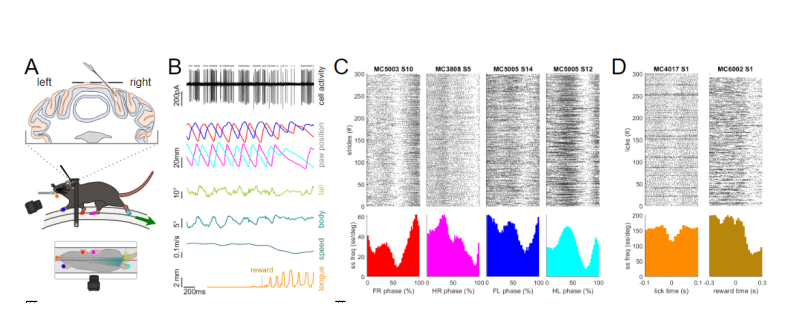
\includegraphics[width=1\linewidth]{Chapters/Figures/chapter3/behavioral_correlations_in_fr.png}
    \caption{Purkinje cells are modulated by multiple limbs. \textbf{A} Stride phases are extracted from positions for each paw by linearly interpolating between swing and stance events.}
    \label{fig:behavioral-correlations}
\end{figure}

\par This aspect of locomotion poses a difficulty when isolating paw contributions to firing rate. Two correlated limbs will have similar tuning functions, and they will be in anti-phase relative to the homolateral pair.

% \subsection{GAMs decompose firing rate into limb tuning}

% ...........................................

Marques, Ramirez et al.~have recently used generalized additive models (GAMs) as a way to disentangle the contributions of multiple correlated limb signals into their individual contributions \cite{ramirez-buriticaNonlinearMixedEncoding2024}.
Under this framework, limb phases are extracted from limb positions by linearly interpolating 2 core segments corresponding to swing and stance periods. The continuous phase for each paw is then binned into multiple basis functions (Figure \ref{fig:gam-methods}A).


To account for behavioral confounds metrics like tail angle, wheel speed, and body angle were included in the models. These can be binarized in similar manner to paw phases and included as regressors in a model of the following form: 


\begin{gather}
\label{fig:behavioral-correlations}
\text{Firing Rate} = \beta_0 + \sum_{i=1}^{N} \sum_{j=1}^{M} \beta_{i,j} \cdot \phi_{i,j} + \epsilon
\intertext{\indent Where:}
  \begin{tabular}{l c l}
    \(\beta_0\)     & : & \(y\) intercept  \\
    \(N\)           & : & number of behavioral regressors \\
    \(M\)           & : & number of bins / basis functions \\
     \(\phi_{i,j}\) & : & basis function for behavioral regression \(i\) bin \(j\) \\
    \(\beta_{i,j}\) & : & model coefficient for behavioral regression \(i\) bin \(j\) \\
    \(\epsilon\)    & : & residuals
  \end{tabular}\nonumber
\end{gather}

and a tuning function is the smoothed collection of \(\beta\) for all \(j\) (\ref{fig:gam-methods}B).

The outputs of the GAM are the coefficients organized in the phase space of each variable, i.e., partial dependency functions (PDPs), that can be interpreted as tuning functions (Figure \ref{fig:gam-methods}C), as well as the predicted firing rate.

\begin{figure}[h]
    \centering
    \includegraphics[width=0.9\linewidth]{example-image}
    \caption{Purkinje cells are modulated by multiple limbs. \textbf{A} Stride phases are extracted from positions for each paw by linearly interpolating between swing and stance events.}
    \label{fig:gam-methods}
\end{figure}

Ramirez et al.~fitted one GAM per recorded Purkinje cell

% \subsection{Emergence of a non-linear component for limb mixing in Purkinje cells}

GAMs also allow specifying non-linear interactions between regressors under the hypothesis that some variance in the firing rate is due to specific combinations of features. In our case, these combinations would occur in a 4 dimensional phase space combined from all paws.
\par 





% \section{Neural decoding}
% Describe the concepts behind neural decoding here, mostly from Glaser and Kording.
% \subsection{Encoding: building pseudo-population firing rates from single-cell recording sessions}
% \subsection{Decoding: statistical metrics for behavioral readouts}
% \subsection{Purkinje cell non-linear mixed representations improve behavioral readouts}
